%% Copyright (c) 2015-2020, RTE (http://www.rte-france.com)
%% See AUTHORS.txt
%% All rights reserved.
%% This Source Code Form is subject to the terms of the Mozilla Public
%% License, v. 2.0. If a copy of the MPL was not distributed with this
%% file, You can obtain one at http://mozilla.org/MPL/2.0/.
%% SPDX-License-Identifier: MPL-2.0
%% This file is part of Dynawo, an hybrid C++/Modelica open source time domain
%% simulation tool for power systems.
\documentclass[a4paper, 12pt]{report}

%% Except where otherwise noted, content in this documentation is Copyright (c)
%% 2015-2019, RTE (http://www.rte-france.com) and licensed under a
%% CC-BY-4.0 (https://creativecommons.org/licenses/by/4.0/)
%% license. All rights reserved.

% Latin Modern fam­ily of fonts
\usepackage{lmodern}

\usepackage[english]{babel}

% specify encoding
\usepackage[utf8]{inputenc} % input
\usepackage[T1]{fontenc} % output

% Document structure setup
\usepackage{titlesec} % To change chapter format
\setcounter{tocdepth}{3} % Add subsubsection in Content
\setcounter{secnumdepth}{3} % Add numbering for subsubsection
\setlength{\parindent}{0pt} % No paragraph indentation

% Change title format for chapter
\titleformat{\chapter}{\Huge\bf}{\thechapter}{20pt}{\Huge\bf}

% To add links on page number in Content and hide red rectangle on links
\usepackage[hidelinks, linktoc=all]{hyperref}
\usepackage[nottoc]{tocbibind}  % To add biblio in table of content
\usepackage{textcomp} % For single quote
\usepackage{url} % Allow linebreaks in \url command
\usepackage{listings} % To add code samples

% Default listings parameters
\lstset
{
  aboveskip={1\baselineskip}, % a bit of space above
  backgroundcolor=\color{shadecolor}, % choose the background color
  basicstyle={\ttfamily\footnotesize}, % use font and smaller size \small \footnotesize
  breakatwhitespace=true, % sets if automatic breaks should only happen at whitespace
  breaklines=true, % sets automatic line breaking
  columns=fixed, % nice spacing -> fixed / flexible
  mathescape=false, % escape to latex false
  numbers=left, % where to put the line-numbers
  numberstyle=\tiny\color{gray}, % the style that is used for the line-numbers
  showstringspaces=false, % do not emphasize spaces in strings
  tabsize=4, % number of spaces of a TAB
  texcl=false, % activates or deactivates LaTeX comment lines
  upquote=true % upright quotes
}

% Avoid numbering starting at each chapter for figures
\usepackage{chngcntr}
\counterwithout{figure}{chapter}

\usepackage{tikz} % macro pack­age for cre­at­ing graph­ics
\usepackage{pgfplots} % draws func­tion plots (based on pgf/tikz)

\usepackage{algorithm} % Add algorithms
\usepackage[noend]{algpseudocode} %  all end ... lines are omitted in algos

\usepackage{amsmath} % Add math­e­mat­i­cal fea­tures
\usepackage{schemabloc} % Add block diagram library (french one)

\usepackage{adjustbox} % Add box for flowchart

\usepackage{booktabs} % for toprule and midrule in tables

\usepackage{tabularx}

\usepackage[nolist]{acronym} % don’t write the list of acronyms.
% Acronyms list
\begin{acronym}
\acro{BDF}{Backward Differentiation Formula}
\acro{BE}{Backward Euler}
\acro{DAE}{Differential Algebraic Equations}
\acro{IDA}{Implicit Differential-Algebraic solver}
\acro{LLNL}{Lawrence Livermore National Lab}
\acro{KINSOL}{Krylov Inexact Newton SOLver}
\acro{NR}{Newton-Raphson}
\acro{PLL}{Phase-Locked Loop}
\acro{SVC}{Static Var Compensator}
\acro{SUNDIALS}{SUite of Nonlinear and DIfferential/ALgebraic equation Solvers}
\acro{WECC}{Western Electricity Coordinating Council}
\end{acronym}

% Syntax highlight
%% Except where otherwise noted, content in this documentation is Copyright (c)
%% 2015-2019, RTE (http://www.rte-france.com) and licensed under a
%% CC-BY-4.0 (https://creativecommons.org/licenses/by/4.0/)
%% license. All rights reserved.

\usepackage{color}

\definecolor{blue}{rgb}{0,0,1}
\definecolor{lightblue}{rgb}{.3,.5,1}
\definecolor{darkblue}{rgb}{0,0,.4}
\definecolor{red}{rgb}{1,0,0}
\definecolor{darkred}{rgb}{.56,0,0}
\definecolor{pink}{rgb}{.933,0,.933}
\definecolor{purple}{rgb}{0.58,0,0.82}
\definecolor{green}{rgb}{0.133,0.545,0.133}
\definecolor{darkgreen}{rgb}{0,.4,0}
\definecolor{gray}{rgb}{.3,.3,.3}
\definecolor{darkgray}{rgb}{.2,.2,.2}
\definecolor{shadecolor}{gray}{0.925}

% **********************************************************************************
% Syntax : Bash (bash)
% **********************************************************************************

\lstdefinelanguage{bash}
{
  keywordstyle=\color{blue},
  morekeywords={
    cd,
    export,
    source},
  numbers=none,
  deletekeywords={jobs}
}

% **********************************************************************************
% Syntax : XML
% **********************************************************************************

\lstdefinelanguage{XML}
{
  morestring=[s][\color{purple}]{"}{"},
  morecomment=[s][\color{green}]{<?}{?>},
  morecomment=[s][\color{green}]{<!--}{-->},
  stringstyle=\color{black},
  identifierstyle=\color{blue},
  keywordstyle=\color{red},
  morekeywords={
    xmlns,
    xsi,
    noNamespaceSchemaLocation,
    type,
    source,
    target,
    version,
    tool,
    transRef,
    roleRef,
    objective,
    eventually}
}

% **********************************************************************************
% Syntax : Modelica (modelica)
% **********************************************************************************
\lstdefinelanguage{Modelica}{
  alsoletter={...},
  morekeywords=[1]{ % types
      Boolean,
      Integer,
      Real},
  keywordstyle=[1]\color{red},
  morekeywords=[2]{ % keywords
    algorithm,
    and,
    annotation,
    assert,
    block,
    class,
    connector,
    constant,
    discrete,
    else,
    elseif,
    elsewhen,
    end,
    equation,
    exit,
    extends,
    external,
    false,
    final,
    flow,
    for,
    function,
    if,
    in,
    inner,
    input,
    import,
    loop,
    model,
    nondiscrete,
    not,
    or,
    outer,
    output,
    package,
    parameter,
    public,
    protected,
    record,
    redeclare,
    replaceable,
    return,
    size,
    terminate,
    then,
    true,
    type,
    when,
    while},
  keywordstyle=[2]\color{darkred},
  morekeywords=[3]{ % functions
    abs,
    acos,
    asin,
    atan,
    atan2,
    Complex,
    connect,
    conj,
    cos,
    cosh,
    cross,
    der,
    edge,
    exp,
    fromPolar,
    imag,
    noEvent,
    pre,
    sign,
    sin,
    sinh,
    sqrt,
    tan,
    tanh},
  keywordstyle=[3]\color{blue},
  morecomment=[l][\color{green}]{//}, % comments
  morecomment=[s][\color{green}]{/*}{*/}, % comments
  morestring=[b][\color{pink}]{'}, % strings
  morestring=[b][\color{pink}]{"}, % strings
}


\usepackage{xspace} % Define typography
\usepackage{dirtree}
\newcommand{\Dynawo}[0]{Dyna$\omega$o\xspace}

\pgfkeys{
/pgf/number format/read comma as period
}

\begin{document}
\chapter*{Illustrative examples for the steady state simulator}

This document presents the results of several simple test cases to illustrate the possibilities of the steady state simulator.

\section*{Phase Shifters in parallel (PhaseShifters)}

The following system is simulated. It is made of a generator (GeneratorPVSignalN), two phase shifter transformers, a transformer, five lines and a PQ load (LoadPQ).\\

\begin{figure}[H]
  \begin{center}
  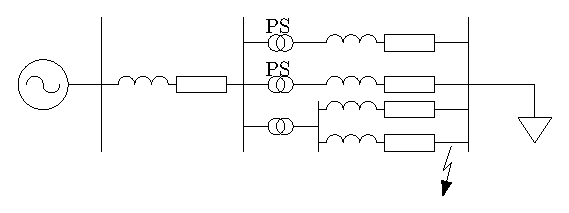
\includegraphics[width=0.8\textwidth]{PhaseShifters/PhaseShifters}
  \end{center}
  \caption{Illustration of the studied system}
\end{figure}

The line is disconnected at t = 30s.\\
Two simulations are done :
\begin{itemize}
\item the two phase shifters have the following time constants t1st = 40s/tNext = 20s;
\item one phase shifter have the following time constants t1st = 20s/tNext = 10s, the other one t1st = 40s/tNext = 20s.
\end{itemize}

The currents in both phase shifters are compared in both cases. One can observe that depending on the time constants of the phase shifter, the steady state after the event is different.\\
\\
This cannot be captured by a fully static simulator, in which all the phase shifters are activated at the same time with an external loop.

\begin{figure}[H]
  \begin{tikzpicture}
    \begin{axis}[xmin = 0, ymin = 0.24, ymax = 0.34, height = 2.3in, legend pos=north east]
        \addplot[color=red!50,line width=0.03in]
        table[x=time,y=PhaseShifter_5_6_phaseShifter_iMonitored]
        {PhaseShifters/curves2010.csv};
        \addplot[color=blue!50,line width=0.03in]
        table[x=time,y=PhaseShifter_5_6_phaseShifter_iMonitored]
        {PhaseShifters/curves4020.csv};
        \legend{20/10, 40/20}
        \end{axis}
  \end{tikzpicture}
  \caption{Current in the first phase shifter [p.u]}
\end{figure}

\begin{figure}[H]
  \begin{tikzpicture}
    \begin{axis}[xmin = 0, ymin = 0.24, ymax = 0.34, height = 2.3in, legend pos=north east]
        \addplot[color=red!50,line width=0.03in]
        table[x=time,y=PhaseShifter_5_7_phaseShifter_iMonitored]
        {PhaseShifters/curves2010.csv};
        \addplot[color=blue!50,line width=0.03in]
        table[x=time,y=PhaseShifter_5_7_phaseShifter_iMonitored]
        {PhaseShifters/curves4020.csv};
        \legend{20/10, 40/20}
        \end{axis}
  \end{tikzpicture}
  \caption{Current in the second phase shifter [p.u]}
\end{figure}

\section*{Simplified HVDC link with AC emulation and phase shifter (HVDC\_PhaseShifter)}

The following system is simulated. It is made of a generator (GeneratorPVSignalN), a phase shifter transformer, four lines, two transformers, a simplified HVDC link with an AC emulation (SimplifiedHVDCACEmulation) and a PQ load (LoadPQ).\\

\begin{figure}[H]
  \begin{center}
  
\includegraphics[width=0.8\textwidth]{HVDC_PhaseShifter/HVDC_PhaseShifter}
  \end{center}
  \caption{Illustration of the studied system}
\end{figure}

The line is disconnected at t = 30s.\\
Two simulations are done :
\begin{itemize}
\item the time constant of the HVDC link is equal to 50s;
\item the time constant of the HVDC link is equal to 1s.
\end{itemize}

One can observe that, in the case where the HVDC link time constant is equal to 50s, its power increases too slowly. As a consequence, the power in the phase shifter is too high for a too long time, which induces a tap change that doesn't happen when the time constant is equal to 1s.\\
\\
This cannot be captured by a fully static simulator, in which the HVDC link has no dynamics (which is equivalent to tFilter=0s).

\begin{figure}[H]
  \begin{tikzpicture}
    \begin{axis}[xmax = 120, height = 3in, legend pos=north east]
        \addplot[color=red!50,line width=0.03in]
        table[x=time,y=PhaseShifter_5_6_phaseShifter_PMonitored]
        {HVDC_PhaseShifter/curves1.csv};

        \addplot[color=blue!50,line width=0.03in]
        table[x=time,y=PhaseShifter_5_6_phaseShifter_PMonitored]
        {HVDC_PhaseShifter/curves50.csv};

        \legend{tFilter = 1s, tFilter = 50s}
        \end{axis}
  \end{tikzpicture}
  \caption{Active power in the phase shifter [p.u]}
\end{figure}

\begin{figure}[H]
  \begin{tikzpicture}
    \begin{axis}[xmax = 120, height = 3in, legend pos=north east]
        \addplot[color=red!50,line width=0.03in]
        table[x=time,y=HVDC_hvdc_P1Pu]
        {HVDC_PhaseShifter/curves1.csv};

        \addplot[color=blue!50,line width=0.03in]
        table[x=time,y=HVDC_hvdc_P1Pu]
        {HVDC_PhaseShifter/curves50.csv};

        \legend{tFilter = 1s, tFilter = 50s}
        \end{axis}
  \end{tikzpicture}
  \caption{Active power in the HVDC link [p.u]}
\end{figure}

\section*{Simplified HVDC link with AC emulation and CLA (HVDC\_CLA)}

The following system is simulated. It is made of a generator (GeneratorPVSignalN), four lines (one is monitored by a current limiter automaton), two transformers, a simplified HVDC link with an AC emulation (SimplifiedHVDCACEmulation) and a PQ load (LoadPQ).\\

\begin{figure}[H]
  \begin{center}
  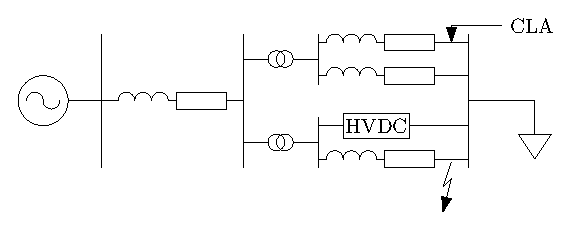
\includegraphics[width=0.8\textwidth]{HVDC_CLA/HVDC_CLA}
  \end{center}
  \caption{Illustration of the studied system}
\end{figure}

The line is disconnected at t = 30s.\\
Two simulations are done :
\begin{itemize}
\item the time constant of the HVDC link is equal to 60s;
\item the time constant of the HVDC link is equal to 30s.
\end{itemize}

One can observe that, in the case where the HVDC link time constant is equal to 60s, its power increases too slowly. As a consequence, the current in the line that is monitored by the CLA is too high for a too long time, which induces a line disconnection that doesn't happen when the time constant is equal to 30s.\\
\\
This cannot be captured by a fully static simulator, in which the HVDC link has no dynamics (which is equivalent to tFilter=0s).

\begin{figure}[H]
  \begin{tikzpicture}
    \begin{axis}[xmax = 120, height = 3in, legend pos=south east]
        \addplot[color=red!50,line width=0.03in]
        table[x=time,y=HVDC_hvdc_P1Pu]
        {HVDC_CLA/curves30.csv};

        \addplot[color=blue!50,line width=0.03in]
        table[x=time,y=HVDC_hvdc_P1Pu]
        {HVDC_CLA/curves60.csv};

        \legend{tFilter = 30s, tFilter = 60s}
        \end{axis}
  \end{tikzpicture}
  \caption{Active power in the HVDC link [p.u]}
\end{figure}

\begin{figure}[H]
  \begin{tikzpicture}
    \begin{axis}[xmax = 120, height = 3in, legend pos=south east]
        \addplot[color=red!50,line width=0.03in]
        table[x=time,y=NETWORK__BUS____7-BUS___10-2_AC_iSide2]
        {HVDC_CLA/curves30.csv};

        \addplot[color=blue!50,line width=0.03in]
        table[x=time,y=NETWORK__BUS____7-BUS___10-2_AC_iSide2]
        {HVDC_CLA/curves60.csv};

        \legend{tFilter = 30s, tFilter = 60s}
        \end{axis}
  \end{tikzpicture}
  \caption{Current in the remaining AC line [A]}
\end{figure}

\section*{Load restoration (LoadRestoration)}

The following system is simulated. It is made of a generator (GeneratorPVSignalN), two transformers, three lines and a restorative alpha beta load (LoadAlphaBetaRestorative).\\

\begin{figure}[H]
  \begin{center}
  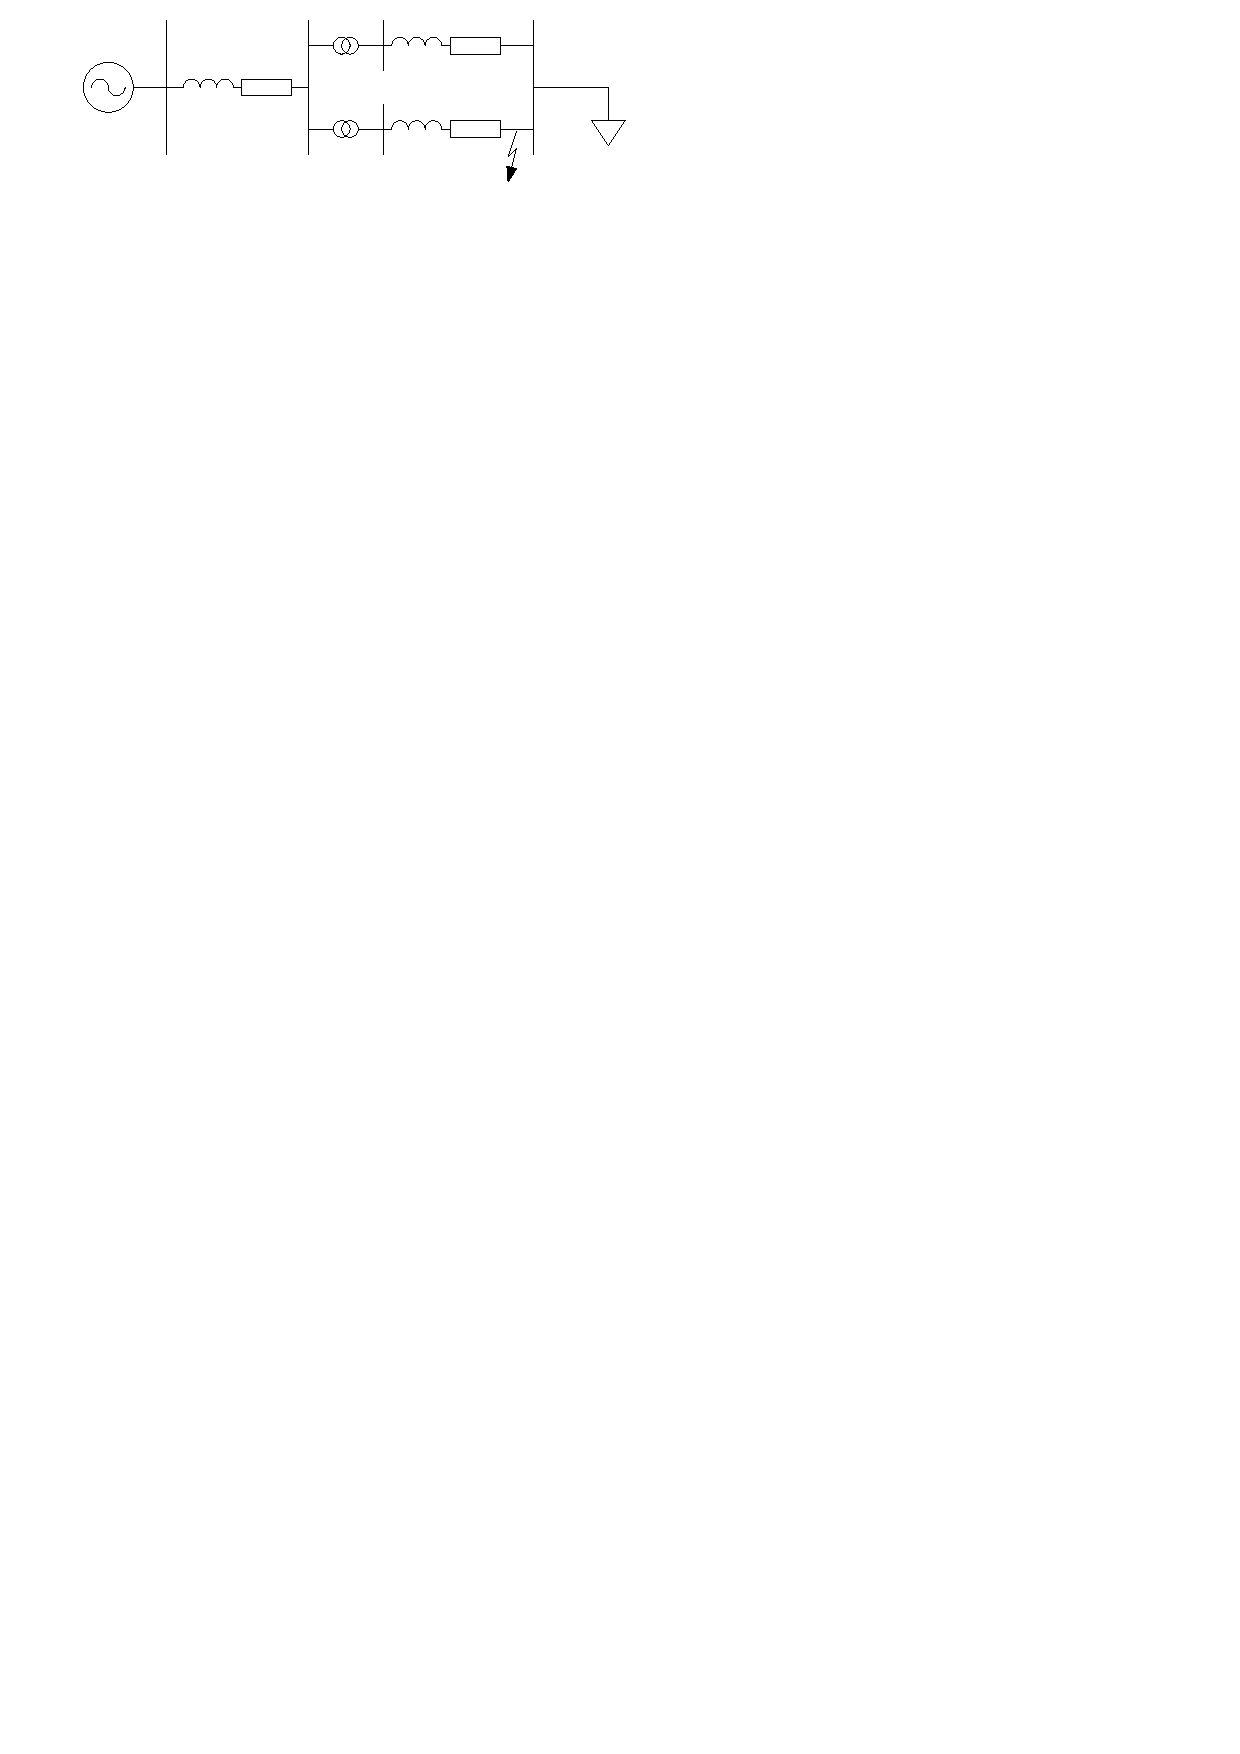
\includegraphics[width=0.8\textwidth]{LoadRestoration/LoadRestoration}
  \end{center}
  \caption{Illustration of the studied system}
\end{figure}

The line is disconnected at t = 30s.\\
Two simulations are done :
\begin{itemize}
\item the load restoration is complete (UMinPu = 0);
\item the load restoration is not complete (the voltage goes below UMinPu = 0.95 p.u, which decreases the load active power following an alpha-beta behaviour).
\end{itemize}

One can notice that when the restoration is complete, the simulation fails, as would a purely static simulation (power flow).

When the restoration is not complete, the active power of the load is below the maximum transferrable power. As a consequence, the simulation succeeds.

\end{document}
